\documentclass[
    twoside=false,
    twocolumn=true,
    fontsize=11pt,
]{scrarticle}
\usepackage{xcolor}
\definecolor{seeblau}{HTML}{00A9E0}
\definecolor{seegrau}{HTML}{9AA0A7}

\definecolor{seeblau1}{HTML}{CCEEF9}
\definecolor{seeblau2}{HTML}{A6E1F4}
\definecolor{seeblau3}{HTML}{59C7EB}
\definecolor{seeblau4}{HTML}{00A9E0}
\definecolor{seeblau5}{HTML}{008ECE}


\usepackage{graphicx}
\usepackage{amsmath}
\usepackage{subcaption}
\usepackage{wrapfig}
\usepackage[english]{babel}
\usepackage{blindtext}
\usepackage{microtype}
\usepackage{siunitx}
\usepackage[utf8]{inputenc}
\usepackage{csquotes}
\usepackage{nicefrac}
\usepackage[T1]{fontenc}
\usepackage{amsfonts}
\usepackage{amssymb}
\usepackage{tikz}

\usepackage{siunitx}

\usepackage{libertinus, libertinust1math}
\usepackage{roboto}

\setkomafont{disposition}{\normalfont\sffamily}


% not recommended with KOMA-script
% make table of contents sans-serif
% \usepackage{tocloft}
% \renewcommand\cftchappagefont{\normalfont}
% \renewcommand\cftchapfont{\normalfont}
% \renewcommand\cftchappresnum{\bfseries}
% \renewcommand\cftchapaftersnum{}
% \renewcommand{\cftchapfont}{\sffamily}
% \renewcommand{\cftsecfont}{\sffamily}
% \renewcommand{\cftsubsecfont}{\sffamily}
% \renewcommand{\cftchappagefont}{\sffamily}
% \renewcommand{\cftsecpagefont}{\sffamily}
% \renewcommand{\cftsubsecpagefont}{\sffamily}

% caption
\usepackage{caption}
\captionsetup{
	% font={sf},
	labelfont={sf, bf, color=seeblau},
	labelsep=quad,
	labelformat=simple,
}

% links
\usepackage{hyperref}
\hypersetup{
	colorlinks=true,
	linkcolor=seeblau,
	citecolor=seeblau,
	urlcolor=seeblau,
	% hidelinks=true
}

% bibliography
\usepackage[
	style=numeric-comp, % comp = compressed 4,5,6,7 -> 4-7
	sorting=none,		% Sort by appearance
	% autocite = superscript,
	% backref=true,
	hyperref=true,
	url=true,
	maxbibnames=100
]{biblatex}
\DefineBibliographyStrings{english}{%
    backrefpage  = {see p.}, % for single page number
    backrefpages = {see pp.} % for multiple page numbers
}

% remove issue
\AtEveryBibitem{%
  \clearfield{number}
}

\usepackage{float}
% \floatplacement{figure}{h}
% \floatplacement{table}{H}

% loosen float placement rules
\renewcommand{\topfraction}{0.8}
\renewcommand{\bottomfraction}{.8}
\renewcommand{\textfraction}{0.1}
\renewcommand{\floatpagefraction}{.9}
% make floats less likely to be placed on a separate page
\setcounter{totalnumber}{9}
\setcounter{topnumber}{9}
\setcounter{bottomnumber}{9}

% decrease space between floats and text
\setlength{\textfloatsep}{0.5cm}
\setlength{\floatsep}{0.5cm}


\usepackage{adjustbox}

\usepackage{datetime}
\newdateformat{dotdate}{
	\twodigit{\THEDAY}.\twodigit{\THEMONTH}.\THEYEAR
}
\newdateformat{monthyeardate}{%
  \monthname[\THEMONTH] \THEYEAR}


% header and footer
\usepackage[
  markcase=noupper
]{scrlayer-scrpage}% activates pagestyle scrheadings automatically
\clearpairofpagestyles
\setkomafont{pageheadfoot}{\normalfont\sffamily}
\setkomafont{pagenumber}{\normalfont\sffamily}
% \chead*{\color{seegrau} Draft \dotdate\today}
\ofoot*{\pagemark}
\ohead*{\rightmark}


\usepackage{ifthen}
\newcommand{\markieren}[4]{
    \ifthenelse{\equal{#1}{}}{}{\adjustbox{padding=3pt, bgcolor=seeblau1, margin=-1pt}{\strut{\sffamily\robotoMedium{#1}}}\\}
    \ifthenelse{\equal{#2}{}}{}{\adjustbox{padding=3pt, bgcolor=seeblau2, margin=-1pt}{\strut{\sffamily\robotoMedium{#2}}}\\}
	\ifthenelse{\equal{#3}{}}{}{\adjustbox{padding=3pt, bgcolor=seeblau3, margin=-1pt}{\strut{\sffamily\robotoMedium{#3}}}\\}
	\ifthenelse{\equal{#4}{}}{}{\adjustbox{padding=3pt, bgcolor=seeblau4, margin=-1pt}{\strut{\sffamily\robotoMedium{#4}}}}
}

\addbibresource{literature.bib}

\begin{document}

\title{title}
\subtitle{subtitle}
\author{Aurel Müller-Schoenau, Leon Oleschko}
\date{\dotdate\today}


% make a custom title page
\begin{titlepage}
    \sffamily
    \vspace*{3cm}
    {
        \fontsize{32}{32}
        \markieren{}{Evanescent light scattering}{Optical Tweezers}{Random Walk}
    }
    \vspace{.25cm}\\
    {
        \Large
        Aurel Müller-Schoenau, Leon Oleschko\\
        Supervised by Krishna Kumar, Karthika
        \vspace{.05cm}\\
        13.11.2024
        \vspace{.25cm}\\
        \normalsize
        Physikalisches Fortgeschrittenenpraktikum 2\\
        Universität Konstanz
    }
    \vfill
    {
        \normalfont\normalsize
        This experiment is determined to investigate the behaviour of a particle undergoing diffusion in the form of Brownian motion both with and without a constrain imposed by the electric field of optical tweezers. Its motion was tracked in the horizontal plane using a microscope. The results make it possible to estimate the diffusion coefficient, which coincides with the theoretical result calculated for an aqueous solution, as well as the effective potential created by the optical tweezers. To measure vertical movements, Total Internal Reflection Microscopy is used in to determine the vertical diffusion movement of the particle as well as the height-dependent diffusion coefficient close to a wall. The measurement was partly successful and qualitatively matches the theoretical model. Curiously, the fit imiplies that the characteristic length of the evanescent field was determined incorrectly. The TIRM results show that forces at the order of a few dozen femto-Newtons can be measured using this method. An attempt to determine the particle mass from the effective gravity failed due to poor measurement results.
    }
    \vfill
    \begin{flushright}
        Available at \url{www.github.com/leoole100/fp2}.
    \end{flushright}
\end{titlepage}

\section{Introduction}
Using the statistics of the random walk small forces can be measured.
This is demonstrated on colloidal particles in an aqueous solution.
Forces are applied using optical tweezers and the position is measured with different microscopy techniques.


% \subsection{Physical Principles}
% kompakten Zusammenstellung der physikalischen Grundlagen


\section{Methods}
\begin{figure}
    \centering
    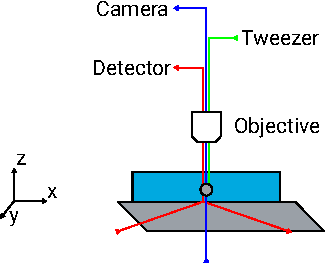
\includegraphics{figures/setup.pdf}
    \caption{Schematic of the experimental setup. Optical tweezers in green, transmission light microscopy in blue and total internal reflection microscopy in red.}
    \label{fig:setup}
\end{figure}
This experiment operates with light on small particles (in the range of \SI{1}{\micro m} \cite{instructions}) in an aqueous solution.
This is shown in \autoref{fig:setup} as the gray circle in the blue box. \\
Using a optical tweezers the particle can be trapped.
This results in a 3-dimensional harmonic potential, which is proportional to the tweezers laser power.
The laser power is continuous (in a used interval) with a unlabeled readout on the laser.
This is value is henceforth referred to as \emph{trap strength}.

To directly observe the particle transmission light microscopy is used.
For this a blue led is used to illuminate the particle from below.
This allows the particle position to measured in $x$ and $y$ direction.

To measure the position in $z$ direction, total internal reflection microscopy is used.
For this a red laser is totally reflected at the boundary below the aqueous solution to create an evanescent wave.
This wave scatters off the particle into a sensitive photo detector.

% \section{Procedure}

\section{Results}
\subsection{Transmission Light Microscopy}
\begin{figure}
    \centering
    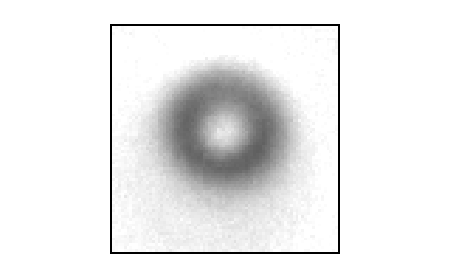
\includegraphics{figures/01_01_1_particle.pdf}
    \caption{Transmission light microscopy of a observed particle. The radius of the particle is \SI{14(2)}{px}, equivalent to \SI{1.86(27)}{\micro m}.}
    \label{fig:01particle}
\end{figure}
In the first section of the experiment, the particles were observed using a transmission light microscope setup.
For this images with a resolution of $600\times 800$\si{px} were recorded with a frequency of \SI{10}{Hz} for \SI{10}{min}.
The magnification of the microscope was assumed to be \SI{0.13319672}{\micro m/px} \cite{instructions}, this is the main systematic error of this measurement, as the scale changes with focus.

The images were normalized with a black (illumination off) and white (illumination on, particle not in frame) reference image, to remove the influence of dust on the imaging elements.
The particle that was used for this experiment is shown in \autoref{fig:01particle}, after the normalization.\\
From this the radius of the particle was estimated to be \SI{1.86(27)}{\micro m}.

\begin{figure*}
    \centering
    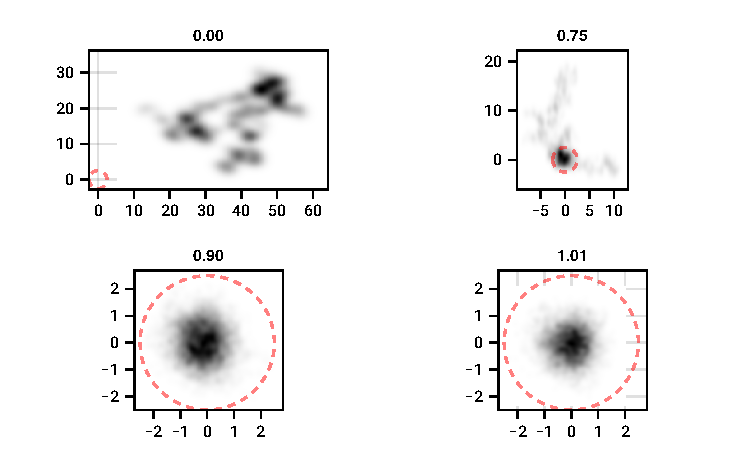
\includegraphics{figures/01_03_1_bivariate.pdf}
    \caption{Density of recorded particle positions, grouped by optical trap stiffness. The red circle indicates the approximate radius of the optical trap \SI{2.5}{\micro m}.}
    \label{fig:01bivariate}
\end{figure*}
To determine the trajectory $\vec r(t)$ of the particle, an effective center of mass was calculated for each frame:
\begin{equation}
    \vec{r}(t) = \iint \vec{r} \; \left(1-I(\vec{r}, t)\right)^2 d\vec{r}    
\end{equation}
The density of the resulting trajectory is shown in \autoref{fig:01bivariate} for different optical trap stiffnesses.
The approximate effective region of the optical trap is drawn as a red circle.

For the trap stiffness of \SI{0}{}, the particle is free to wander around, for the higher stiffnesses (\SI{0.90}{}, \SI{1.01}{}) the particle is mostly confined to the trap.\\
For a weak trap (\SI{0.75}{}) the particle is still mostly confined to the trap, but can escape the linear trap region and randomly wander around, until it is recaptured by the trap.
This happened multiple times during the shown measurement.

\begin{figure}
    \centering
    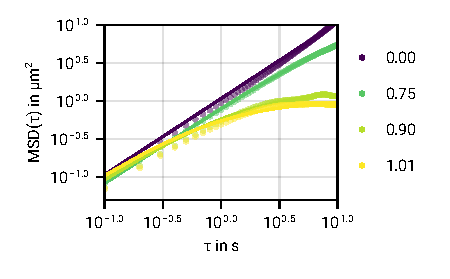
\includegraphics{figures/01_02_2_msd.pdf}
    \caption{Mean Square Displacement for different optical trap stiffnesses, fit: \autoref{eq:01_mdl_msd}}
    \label{fig:01msd}
\end{figure}
\subsection*{Mean Square Displacement}
A method to describe the trajectory of a random walk is the mean square displacement (MSD) \cite{wiki:msd}.
This is defined as the average of the squared distance of the particle from the starting point \cite{wiki:msd}:
\begin{equation}
    \text{MSD}(t) = \frac{1}{N} \sum_i^N \left( x_i\left(t\right) - x_i\left(0\right) \right)^2 
\end{equation}
Here a different implementation using the autocorrelation of the velocity was used, to achieve a more stable result.
This was implemented by \cite{jl:msd}.
The resulting MSD for different optical trap stiffnesses is shown in \autoref{fig:01msd}.

The MSD can be described by the following combination model:
\begin{equation}
    \frac{1}{\text{MSD}(\tau)} = \frac{1}{D_0 \tau} + \frac{1}{\text{MSD}(\infty)}
    \label{eq:01_mdl_msd} 
\end{equation}

For a free particle the $\text{MSD}(\infty)=\infty$ and the MSD grows linearly with $D_0$ over time \cite{wiki:msd,instructions}.\\
The diffusion Coefficient $D_0$ estimated using the fit is shown in \autoref{tab:01spring}.
It is equivalent to the theoretical value of $D_0 = \frac{k_B T}{6 \pi \eta r} = \SI{0.122(18)}{\micro m ^2 / s}$ \cite{instructions}, with $r = \SI{1.86(27)}{\micro m}$ and $\eta = \SI{0.955}{mPa\cdot s}$ \cite{n:water}.
The error in the magnification of the microscope does additionally increase the uncertainty in the measurement.

For a confined particle the MSD reaches a plateau at $\text{MSD}(\infty)$ \cite{instructions}.
This happens for the higher trap stiffness (\SI{0.90}{}, \SI{1.01}{}).
From this the effective spring constant of the optical trap can be estimated $k_{\text{MSD}(\infty)} = \frac{2 k_B T}{\text{MSD}(\infty)}$ \cite{instructions},
the values are shown in  \autoref{tab:01spring} and \autoref{fig:01spring}.\\
For the lower measured spring stiffness (\SI{0.75}{}), the MSD does not reach a plateau, as it partially escapes the trap and wanders around (see \autoref{fig:01bivariate}), behaving like a free particle.\\
Therefore this procedure is not adequate for such low spring stiffnesses.

\begin{table}
    \centering
    \begin{tabular}{r|l|l|l}
        Stiffness & $D_0$ in \SI{}{\micro m^2/s}& $k_{\text{MSD}(\infty)}$ & $k_V$ \\
        \hline        
        \SI{0}{}    & \SI{0.10728(93)}{}    & NA                & \SI{0}{} \\
        \SI{0.75}{} & \SI{0.07793(03)}{}    & NA                & \SI{0.9011(45)}{}\\
        \SI{0.90}{} & \SI{0.0678(24)}{}     & \SI{6.471(62)}{}  & \SI{4.7177(62)}{}\\
        \SI{1.01}{} & \SI{0.05384(08)}{}    & \SI{8.968(23)}{}  & \SI{6.021(12)}{}\\
    \end{tabular}
    \caption{Estimated diffusion constant and spring constant in \SI{}{\nano N / m}.}
    \label{tab:01spring}
\end{table}
\subsubsection*{Potential}
A more detailed analysis can be done by looking at the distribution of the particle positions.
For this the probability density function (PDF) of the particle positions has to be estimated.
This is done using kernel density estimation (KDE) with a Gaussian kernel \cite{jl:kde}.
The resulting 2-dimensional PDF is shown in \autoref{fig:01bivariate}.\\
As the density is small for large parts of the explored 2d space, the data is reduced by aggregating along the image coordinates $x$ and $y$.
As the Potential should by rotationally symmetric, the data from the $x$ and $y$ axis should not significantly deviate.

\begin{figure}
    \centering
    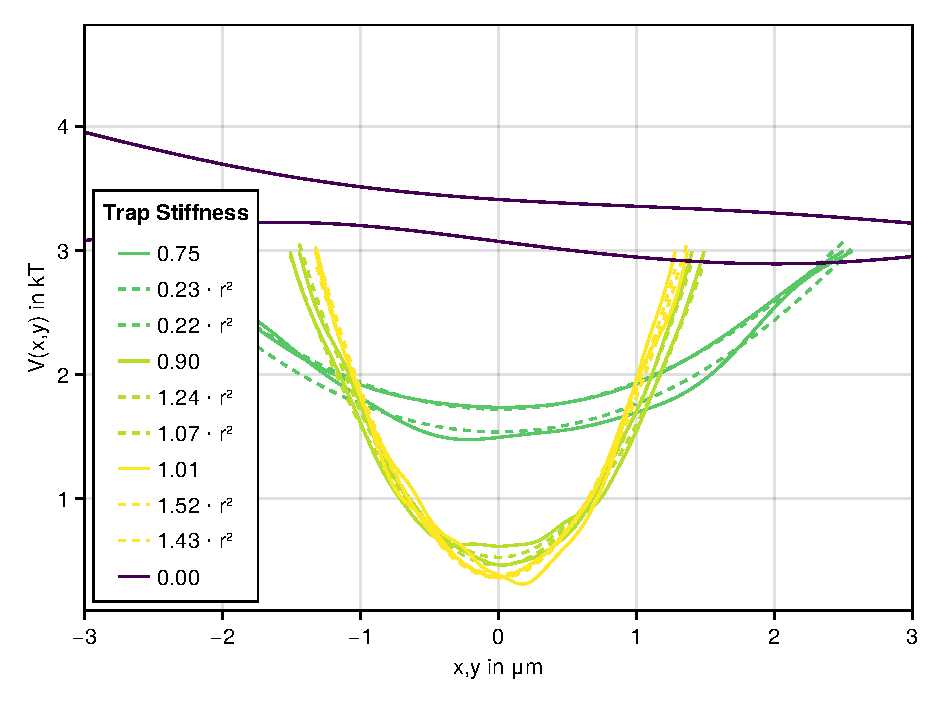
\includegraphics{figures/01_03_3_axis.pdf}
    \caption{Measured Potential, with quadratic fit.}
    \label{fig:01potential}
\end{figure}
\begin{figure}
    \centering
    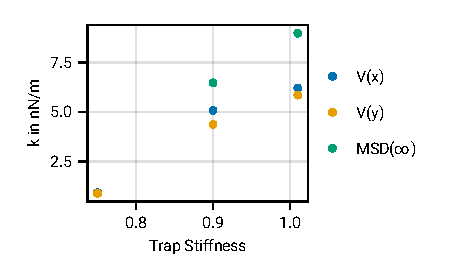
\includegraphics{figures/01_03_4_spring_constants.pdf}
    \caption{Differently measured spring constants.}
    \label{fig:01spring}
\end{figure}
Using the Maxwell Boltzmann relations \cite{instructions}, the potential at a position $p$ can be calculated from the PDF:
\begin{equation}
    V(p) = - \frac{\log{\text{PDF}(p)}}{k_B T}
    \label{eq:pot_boltzmann}
\end{equation}
The resulting potential is shown in \autoref{fig:01potential} for different trap stiffnesses.
The parts of the measurements with a $\text{PDF}(x)>0.05$ are used for a quadratic fit, to estimate the effective spring constant.
The results are shown in \autoref{fig:01spring} and \autoref{tab:01spring} and are in the same order of magnitude, as the estimated spring constant from the MSD.

For the lower spring constant of \SI{0.75}{}, the potential begins quadratically, but flattens after approximately \SI{2.5}{\micro m}.
This is due to the limited size of the trap, but the spring constant can still be estimated.

This method allows for the measurement of a spring constant as low as \SI{0.9011(45)}{\nano N /m}, which means over the used length scales that forces in the order of \SI{1}{\femto N} can be measured.

\subsection{Total Internal Reflection Microscopy}
\emph{Note: Some references in \cite{instructions} led to nowhere, which caused some confusion.}

To measure the particle movement in the vertical direction, \textit{Total Internal Reflection Microscopy} was used: A laser beam is totally reflected at the glass-water boundary below the particle. The resulting evanescent field decays exponentially in the $z$ direction, which means the intensity of the light scattered by the particle allows for precise position measurement on the vertical axis.\\
The scattered light intensity was measured with a frequency of \SI{1}{kHz} for \SI{15}{min}.


\subsubsection*{Position and Diffusion Coefficient}
\begin{figure}
    \centering
    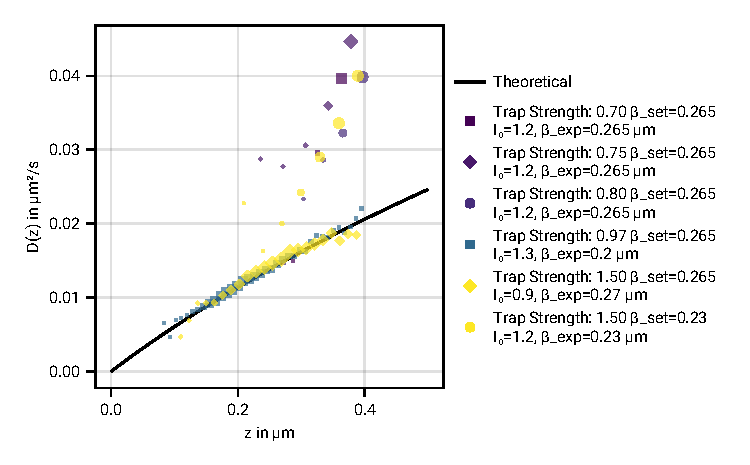
\includegraphics{figures/02_04_01_diffusion.pdf}
    \caption{Estimated diffusion coefficient for different measurements. With a theoretical model corresponding to \autoref{eq:D_Brenner_approx}.}
    \label{fig:D_of_z}
\end{figure}

The $z$ distance between particle and wall can be calculated using the formula \cite{instructions}
\begin{equation}
 \label{eq:calculate_z}
 z = \beta \left(\log(I_0) - \log(I)\right)
\end{equation}
where $I$ is the scattered light intensity and $I_0$ is the maximum possible intensity, i.e. $I(z=0)$, when the particle touches the glass surface. $\beta$ is the characteristic length of the evanescent field which can be calculated from the angle of incident of the reflected beam.\\
The $z$-dependent diffusion coefficient can be calculated from the position changes $\Delta z$ in a given $z$ interval. For Brownian motion these should be normally distributed with
\begin{equation}
\label{eq:D_delta_t}
 \sigma^2 = 2 \cdot D \cdot \Delta t
\end{equation}
where $D$ is the diffusion coefficient \cite{instructions}. In reality there is an additional component owing to measurement uncertainty which does not depend on $\Delta t$. To eliminate it, the derivative with respect to $\Delta t$ is estimated by calculating \autoref{eq:D_delta_t} for different $\Delta t$.\\
Close to a wall, the diffusion coefficient can be modeled \cite{instructions} by the equation
\begin{equation}
 \label{eq:D_Brenner_approx}
 D(z) = \frac{D_0}{\left(\frac{R}{z}\right) + 0.2 \log\left(\frac{R}{z}\right) + 0.9712}
\end{equation}
with the radius $R$ of the particle and the free diffusion coefficient $D_0$ by the previously measured value.

To compute $z$ using \autoref{eq:calculate_z} the intensity $I_0$ needs to be estimated.
For this, the steps \autoref{eq:calculate_z} and \autoref{eq:D_delta_t} are calculated iteratively with different $I_0$ trying to match \autoref{eq:D_Brenner_approx}. 
The distance dependent diffusion coefficient $D(z)$ obtained using this method is shown in \autoref{fig:D_of_z}. 

Two measurements yield results matching the theoretical model.
For the other measurement series, four of them shown here using $I_0=1$, it was not possible to match the theoretical model from \autoref{eq:D_Brenner_approx} adjusting $I_0$, and even adjusting $\beta$ did not change that. 
The provided MatLab script yields the same results.\\
The success of the $I_0$ estimation procedure does not depend on the trap stiffness nor the set $\beta$ value.

\begin{figure*}
    \centering
    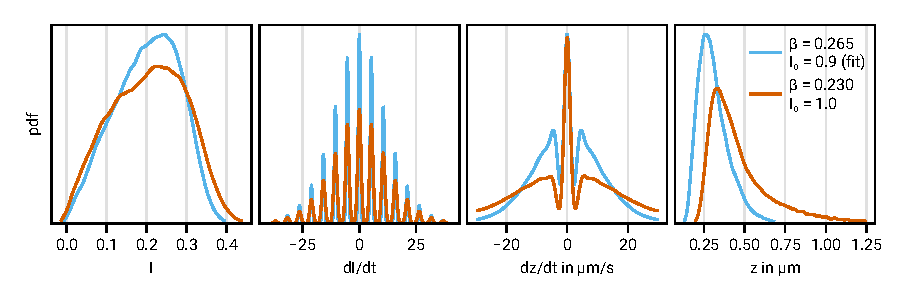
\includegraphics{figures/02_04_02_hist.pdf}
    \caption{Distribution of values for two measurements for the same trap stiffness \SI{1.5}{} but with different $\beta$.}
    \label{fig:pdf_ts_1_5}
\end{figure*}
To investigate this further, the distributions of the measured variables are shown in figure \autoref{fig:pdf_ts_1_5} for a measurement where the procedure was successful and unsuccessful. 
The measurements were conducted with the same trap stiffness of \SI{1.5}{} but different $\beta$ values.\\
The graphs show the estimated PDF for the measured intensity $I$, its derivative as well as the PDF of $z$ and its rate of change. 
As only in one of the two measurements $I_0$ could be estimated, the other one is drawn using $I_0=1$.

The derivative of the intensity shows the limited resolution of the sensor.
The speed distribution $dz/dt$ is expected to be Gaussian.
The peak at $0$ and the neighbouring valleys are a result of measurement quantisation: The $0$-bin of the histogram collects all values around it and no points fall into the neighbouring bins.\\
From the distributions no significant differences were found that could explain why the $I_0$ estimation procedure failed for some measurements.

\subsubsection*{Potential}
\begin{figure}
    \centering
    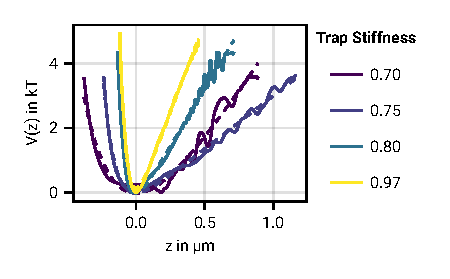
\includegraphics{figures/02_05_01_potential.pdf}
    \caption{Measured Potential for different optical trap stiffnesses.}
    \label{fig:pot_various_ts}
\end{figure}
From the PDF the potential can be calculated using \autoref{eq:pot_boltzmann} like in the previous section. 
The resulting potentials for different optical trap stiffnesses are plotted in \autoref{fig:pot_various_ts}.\\
The potentials are shifted to center around the the mode of $z$ to illustrate the effect of varying the trap stiffness.

The shape of the potential can be modeled as a combination of a effective gravitational force and a Debye screening:
\begin{equation}
 \label{eq:pot_model}
 P(z) = A \; e^{-\kappa z} + z \; F_{g,\text{eff}}
\end{equation}
The characteristic length $\kappa^{-1}$ of the potential close to the wall is called the \textit{Debye Screening Length}. 
$F_{g,\text{eff}}$ is the effective force of gravity acting on the particle inside the solution. 
It is driven by the actual gravitational force but is reduced by buoyancy and increased by the force of the optical trap. \\
For each measurement, the estimated potential was fitted to \autoref{eq:pot_model} to obtain $\kappa$ and $F_{g,\text{eff}}$. 
The results are listed in \autoref{tab:pot_fit}.
\begin{table}
    \centering
    \begin{tabular}{r|c|l}
        stiffness   & effective gravity in \SI{}{\femto N}  & $\kappa^{-1}$ in \SI{}{\nano m} \\
        \hline
        0.70  & \SI{25.88(55)}{} & \SI{260.4(84)}{}\\
        0.75  & \SI{13.47(61)}{} & \SI{ 84.2(12)}{}\\
        0.80  & \SI{29.06(18)}{} & \SI{47.28(83)}{}\\
        0.97  & \SI{46.38(11)}{} & \SI{ 45.6(26)}{}
    \end{tabular}
    \caption{Fit Parameters from the potential. }
    \label{tab:pot_fit}
\end{table}

\begin{figure}
    \centering
    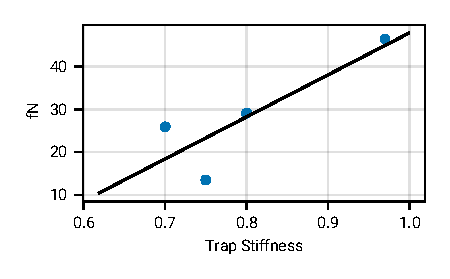
\includegraphics{figures/02_05_02_gravity.pdf}
    \caption{Linear fit of effective gravity for different trap stiffness values.}
    \label{fig:fg_lin}
\end{figure}
\paragraph{Effective Gravity}
The measured effective gravitational force lies in the regime of \SI{10}{\femto N}.
The linear regression of $F_{g,\text{eff}}$ with respect to trap stiffness shown in \autoref{fig:fg_lin} can be used to find the mass of the particle. \\
For this the $0$ of the real trap stiffness is needed, which was estimated to be at \SI{.62(10)}{} units of the non linear trap stiffness.
From this the effective weight of the particle can be estimated to be \SI{10(10)}{\femto N}.
The uncertainty is inconclusively high, as the linear regression is not very good.

\begin{figure}
    \centering
    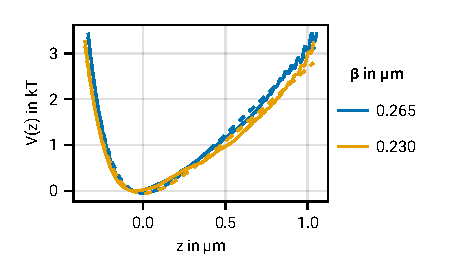
\includegraphics{figures/02_06_01_different_beta.pdf}
    \caption{Measured potential at same trap stiffness \SI{1.5}{}, but different illumination angles resulting in different $\beta$.}
    \label{fig:pot_ts_1_5}
\end{figure}
\paragraph{Influence of $\beta$}
The influence of the angle of incidence of the laser beam on the potential was investigated.
This should not have a influence on the potential.
This is verified by the results shown in \autoref{fig:pot_ts_1_5}.

\pagebreak
\section{Discussion}
The captured image data shows the expected behaviour of a particle trapped inside an approximately harmonic potential performing a random walk. Plotting the mean square displacement over time shows that the particle's movement is restrained to an area around the potential valley. Increasing the trap stiffness restrains the particle more. During one of the measurements the particle escaped the optical trap and moved around freely. The other MSD graphs show the particle behaving as expected, remaining inside the potential well. The diffusion coefficient calculated from the measurements matches the theoretical prediction. The measurement data also allowed for estimation of the potential, illustrating that this method can be used to measure forces in the nano-Newton range.\\
In the second part of the experiment where Total Internal Reflection Microscopy was used to measure the vertical movement of the particle, things did not go so well. The measured intensities were small and therefore prone to quantisation errors due to limitations of the measurement equipment. One issue was poor alignment of the illuminating laser in the beginning of the experiment. This resulted in odd behaviour of the parameter $\beta^{-1}$ corresponding to the characteristic length of the evanescent field, and might be responsible for the low intensity as well. The experiment yielded mixed results for all the measurements conducted in this second part. They can only be considered fully successful in two cases. Here, the analysis routine described above yields proper results for the absolute position of the particle as well as the diffusion coefficient profile close to the wall. The remaining measurement datasets did not allow for that because they cannot fit the theoretical model. In these cases, the measurements failed to provide the information we were looking for. A silver lining is the general resemblence with the theoretically expected shape for the estimated potentials for these measurements assuming $I_0=1$. Combining these findings with the results from the successful measurements allows the determination of the effective gravity and Debye Screening Length in two more cases. However, this yields mixed results yet again. It was not possible to determine the mass of the particle. But the results show that it is possible to measure forces as small as a few dozen femto-Newtons using this method which could be considered a small success. Overall, the second part of the experiment was mostly unsuccessful, owing partly to poor adjustment in the beginning, but also questionable results after applying the data analysis methods meant to resolve this part of the measurement. The setup should be improved to make adjusting the total internal reflection angle easier and more intuitive. The data analysis script could be adjusted to make it more robust in case measurement data does not show the expected behaviour, as in this case the fit results are unreliable which can render entire measurement series useless. Speaking of unreliability, it is difficult to estimate the uncertainty of the results even if everything goes well. The graphs shown in this report illustrate how difficult it can be to make conclusions based off of the fit parameters.\\
Last but not least, the instruction manual \autocite{instructions} for this experiment requires improvement. Some references lead nowhere which caused us some confusion while working on this experiment.


\addcontentsline{toc}{section}{Literature}
\nocite{*}
\printbibliography

\end{document}
